\documentclass[a4paper,12pt]{article}
\usepackage{graphicx} 
\usepackage{amsmath} 

\usepackage{indentfirst}
\usepackage{amsmath} 
\usepackage[varg]{txfonts}
\usepackage{colortbl}
\usepackage{verbatim}
\topmargin=-0.9cm
\oddsidemargin=0.0cm
\evensidemargin=0.0cm
\addtolength{\textheight}{0.5cm}


\definecolor{LemonChiffon}{rgb}{1.,0.98,0.8}
\definecolor{Gold}{rgb}{1.,0.84,0.}
\definecolor{darkblue}{rgb}{0.25,0.,0.95}
\definecolor{lightblue}{rgb}{0.4,0.65,0.95}
\definecolor{grayred}{rgb}{0.7,0.,0.} 
\definecolor{red2}{rgb}{1.0,0.5,0.} 
\definecolor{LemonChiffon}{rgb}{1.,0.98,0.8}
\definecolor{Gold}{rgb}{1.,0.84,0.}
\definecolor{darkblue}{rgb}{0.25,0.,0.95}
\definecolor{lightblue}{rgb}{0.4,0.65,0.95}
\definecolor{RGBblack}{rgb}{0.0,0.0,0.0} 
\def\red{\color{red}}
\def\green{\color{green}}
\def\white{\color{white}}
\def\white{\color{LemonChiffon}}
\def\blue{\color{lightblue}}
\def\gold{\color{Gold}}
\def\black{\color{RGBblack}}



\def\pp{\mathaccent "7F }
\def\p{\mathaccent 95 }


\def\sini {\sin i}
\def\cosi {\cos i}

\def\sino {\sin \Omega}
\def\coso {\cos \Omega}
\def\sinw {\sin \omega}
\def\cosw {\cos \omega}



\begin{document}
\font\norm=cmr12
\font\hugeb=cmb22
\font\isob=cmb18
\font\iso=cmr18
\font\med=cmr14
\font\medb=cmb14
\baselineskip 0.6cm
\parskip\medskipamount
\parskip 0.2cm
\parindent 5mm

%\boldmath

\norm
\hsize 16cm
\vsize 30cm
\newcommand{\bul}{$\bullet \ \ $}
\newcommand{\buu}{\hskip 0.5cm}
\newcommand{\arrow}{$\Rightarrow \ \ $}
\newcommand{\barrow}{\hskip 0.5cm $\Rightarrow \ \ $}
\newcommand{\larrow}{\hskip 0.5cm $\Leftarrow \ \ $}
\newcommand{\hlin}{\vskip 0.5cm}
\newcommand{\hpar}{\vskip 1.0cm}
\newcommand{\nin}{\noindent}
\def\pii{\tilde{\omega}_\circ}

\newcommand{\VV}{$\vec V$ \hskip 0.1cm}
\newcommand{\RR}{$\vec R$ \hskip 0.1cm}

\newcommand{\VVE}{\vec V}
\newcommand{\RRE}{\vec R}


%\pagestyle{empty}
{\centerline{}




{\norm
\vskip 0cm
{{\centerline { {\isob CELESTIAL MECHANICS (Fall 2012): }}}}
\vskip 0.2cm
{{\centerline { {\isob COMPUTER EXERCISES III - SOLUTIONS}}}}

{{\centerline { { (Heikki Salo 26.11.2012)}}}}

\vskip 2cm


These example routines for the solution of the exercises can be copied from

/wrk/hsalo/TM2012\_idl.dir/TM2012\_DEMO3.dir


\newpage
\black
{\medb 8. NUMERICAL INTEGRATION OF TWO BODY MOTION}  


\hlin
{\medb 8.1 Simple example ({\bf inte\_simple.pro}})



\bul A basic main program type procedure for integrating the 2-body
motion in Cartesian coordinates, using either I or II order Taylor
expansion, or Runge-Kutta 4.

\bul Initial values are from the analytical orbit defined by the given
mean anomaly $M$ and by the orbital elements $a, \epsilon$.  Units are set by
$\mu=1$

\bul Integration related paramaters are the step-size $dt$, given
relative to orbital period, and the duration of integration $t_{max}$

\bul The calculated orbit is plotted every $ntul$ steps
 

\bul The energy  and angular momentum (per unit mass) are calculated
before and after the integration. Also printed is the relative change of $h$ and $|\vec k|$ per
orbit.

\bul The function subroutine needed by RK4 procedure is {\bf inte\_simple\_func.pro}. The extra variables (in this case just $\mu$) between the main program and this function are passed via {\em common} statement


{\scriptsize \red
\verbatiminput{inte_simple.pro}
}
\black

\hlin
Function subroutine in {\bf inte\_simple\_func.pro}
{\scriptsize \red
\verbatiminput{inte_simple_func.pro}
}\black


\bul There is also a subroutine version named {\bf inte\_simple\_f.pro}. This uses as defaults: eks=0.5, RK4, dt=0.01 period. Each of these can be changed with a corresponding keyword


\newpage

Example \framebox{\tt inte\_simple\_demo.pro}, which calls {\tt inte\_simple\_f.pro}

 
{\scriptsize 
\begin{verbatim}



psdirect,program+'_1',ps,/color
inte_simple_f,eks=0.5,dt=0.01,choice=1
psdirect,program+'_1',ps,/color,/stop

method=Taylor I   dt/PER=     0.010000000
initial h and k:     -0.50000005      0.86602539
final   h and k:     0.067630238       1.3669949
dh/|h| and dk/|k| per orbit      0.11352605     0.057846982










psdirect,program+'_2',ps,/color
inte_simple_f,eks=0.5,dt=0.01,choice=2
psdirect,program+'_2',ps,/color,/stop

method=Taylor II  dt/PER=     0.010000000
initial h and k:     -0.50000005      0.86602539
final   h and k:     -0.45505289      0.87362013
dh/|h| and dk/|k| per orbit    0.0089894314   0.00087696563
IDL> psclose










psdirect,program+'_3',ps,/color
inte_simple_f,eks=0.5,dt=0.01
psdirect,program+'_3',ps,/color,/stop

method=RK4        dt/PER=     0.010000000
initial h and k:     -0.50000005      0.86602539
final   h and k:     -0.50014636      0.86598613
dh/|h| and dk/|k| per orbit  -2.9261253e-05  -4.5326194e-06


\end{verbatim}
}

\vspace{-18cm}

\hspace{8cm} 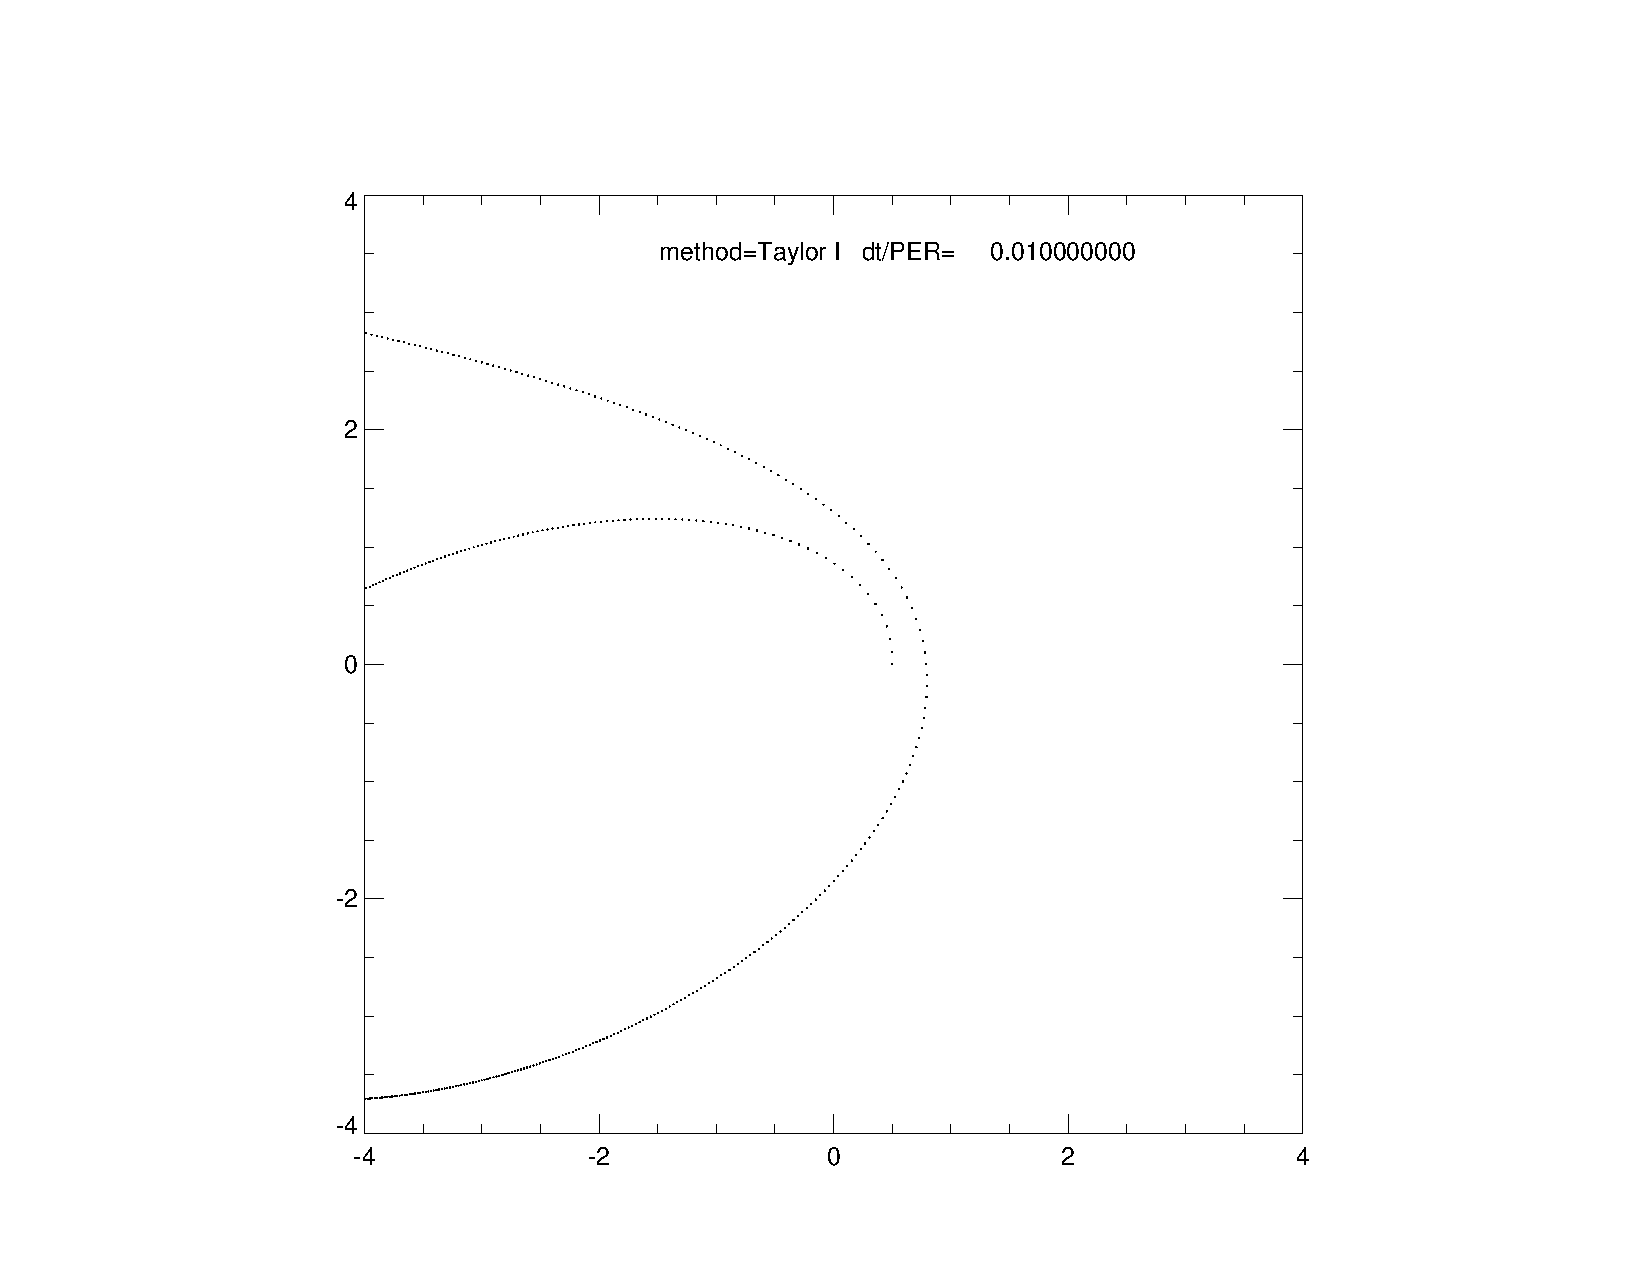
\includegraphics[angle=0,width=0.35\paperwidth]{inte_simple_taylor1.pdf}

\hspace{8cm} 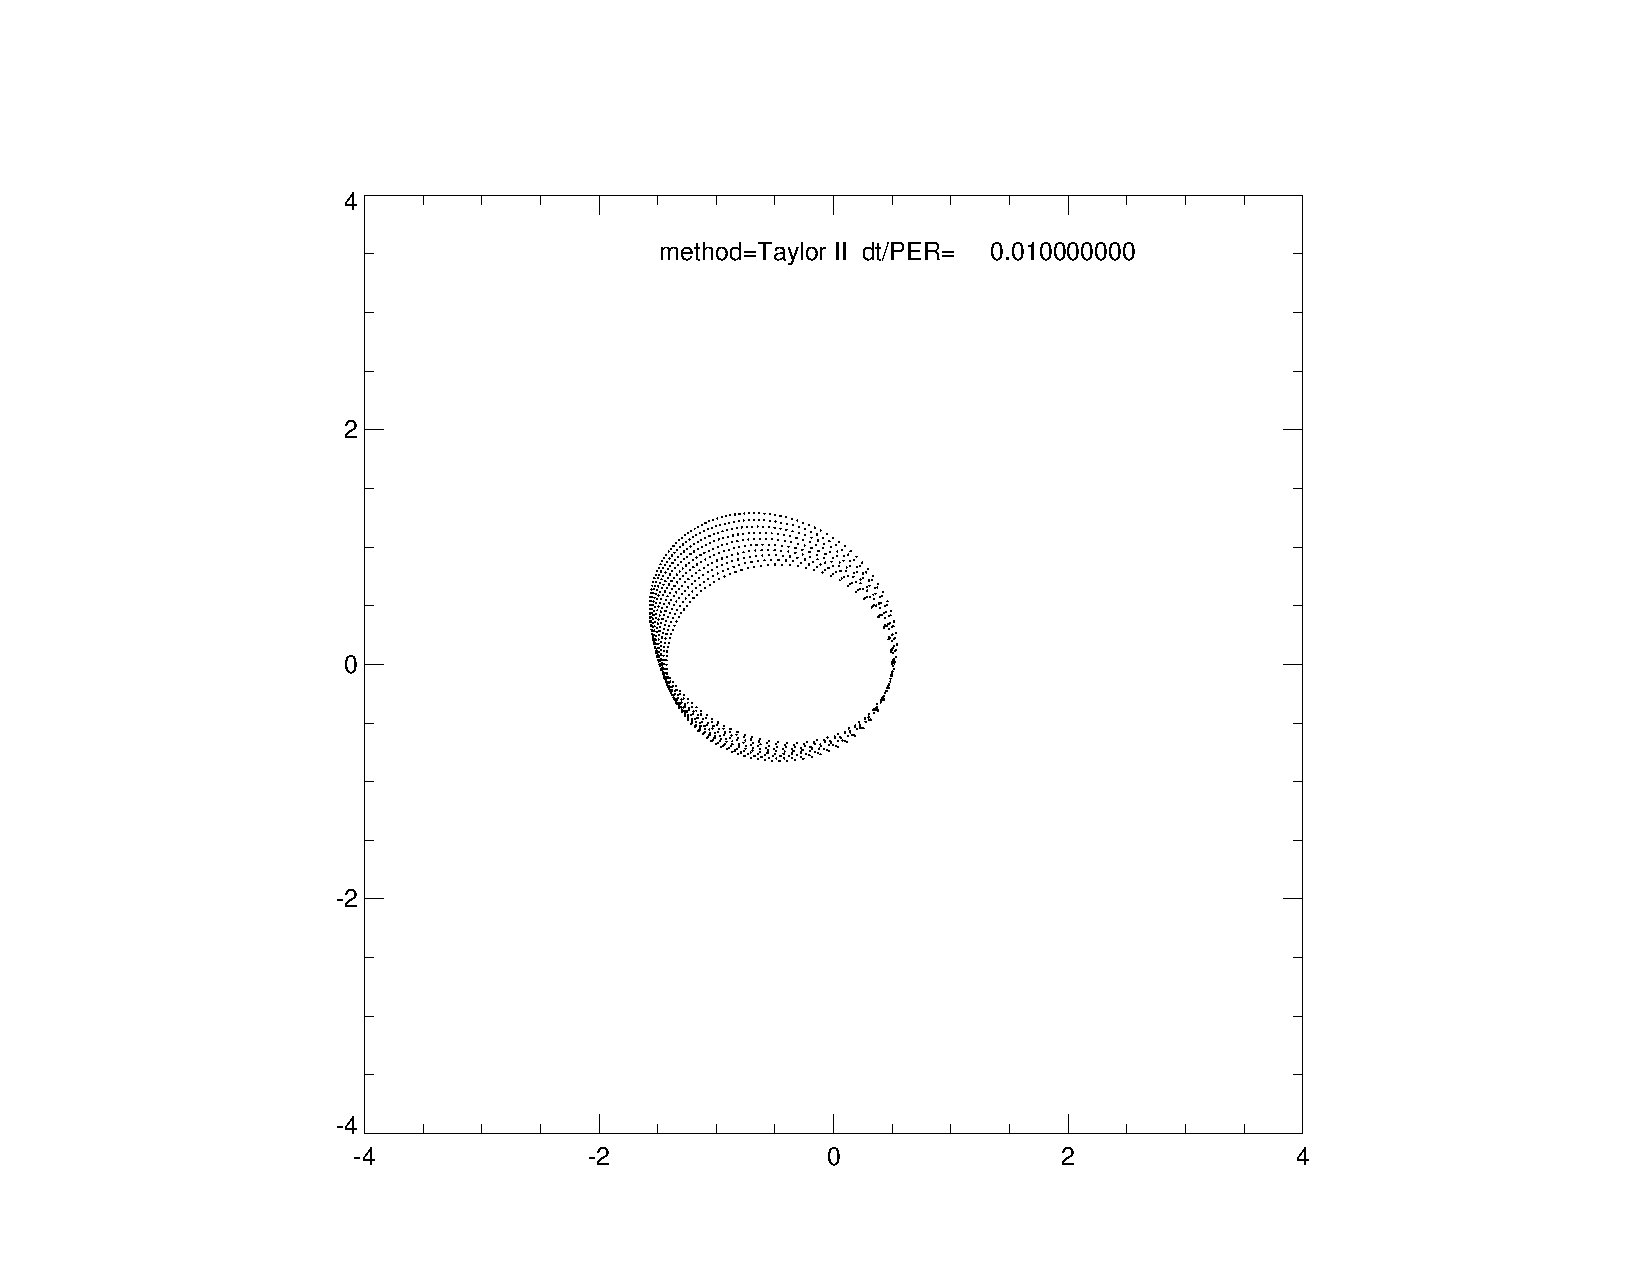
\includegraphics[angle=0,width=0.35\paperwidth]{inte_simple_taylor2.pdf}

\hspace{8cm} 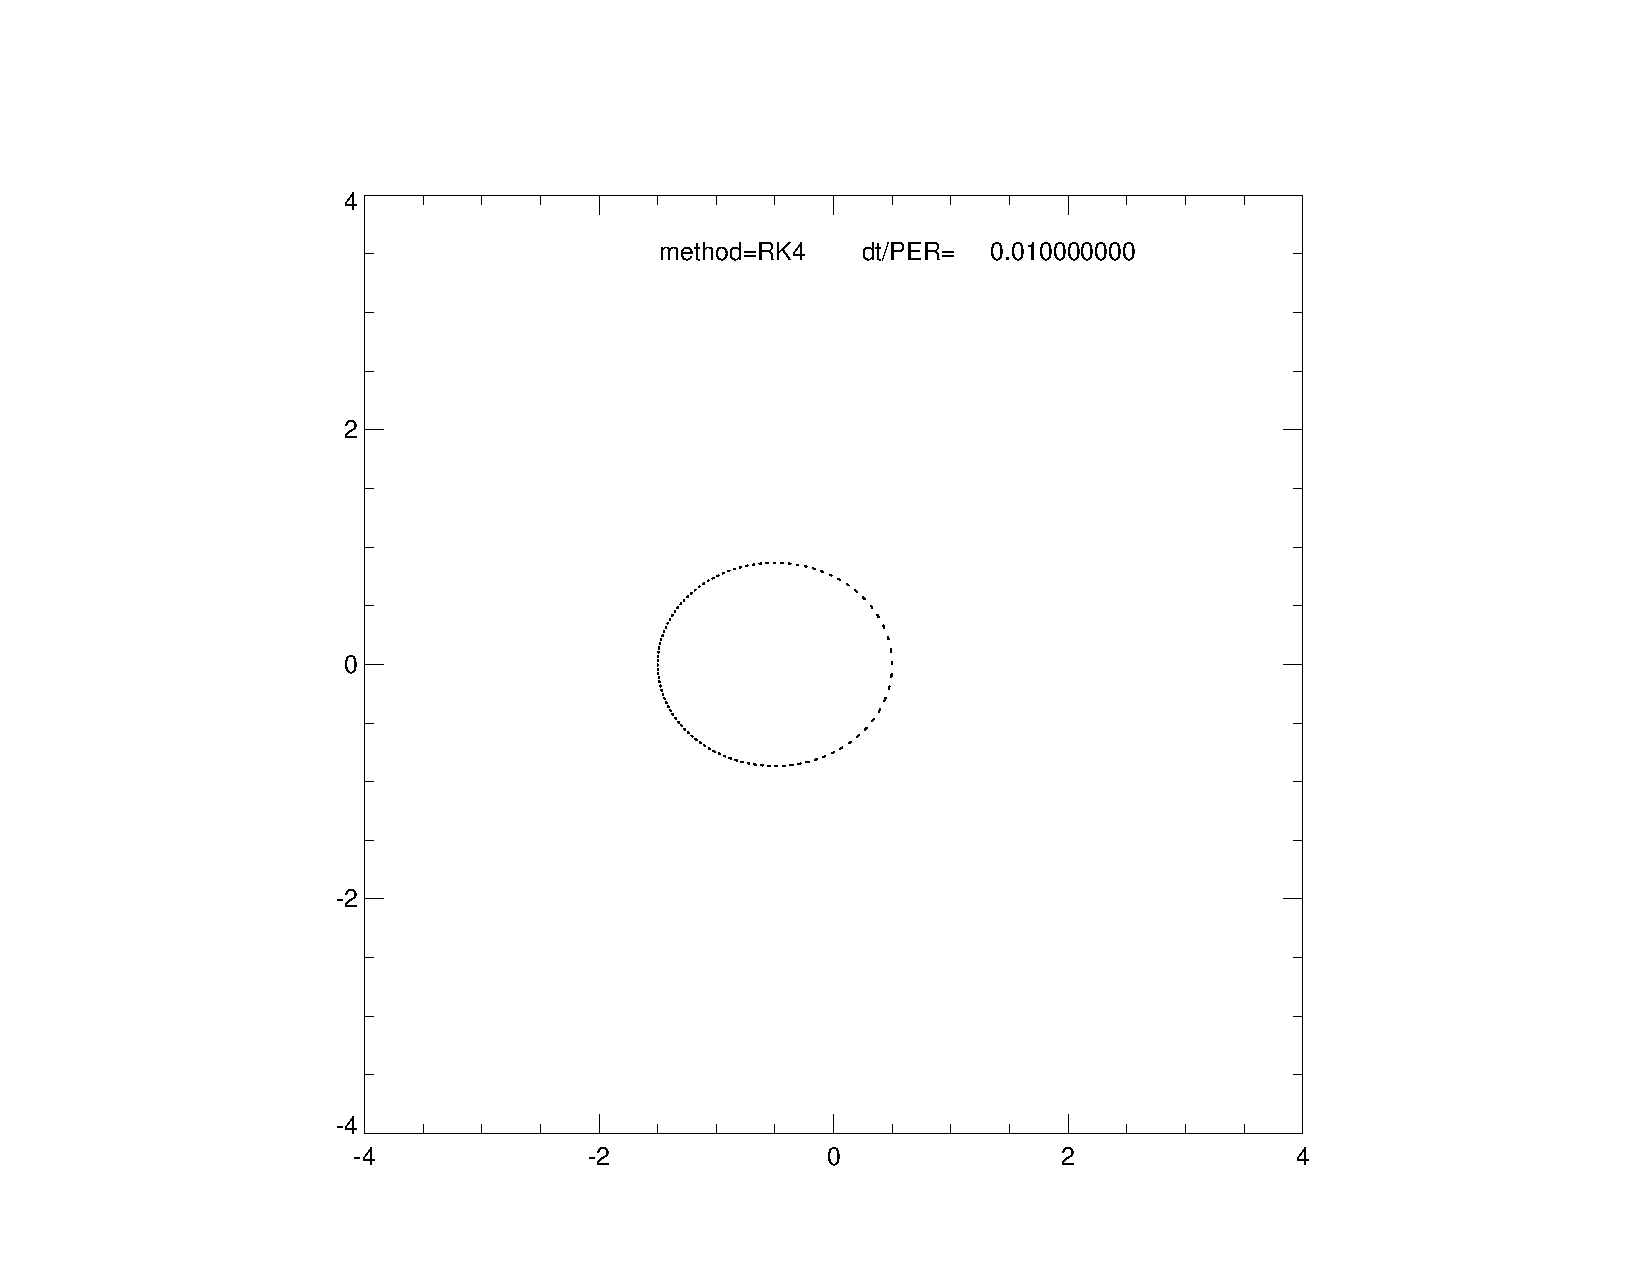
\includegraphics[angle=0,width=0.35\paperwidth]{inte_simple_rk4.pdf}


%*************************************************************************

\newpage

\black

{\medb 8.2 More sophisticated example ({\bf rk\_inte1.pro}})

\bul subroutine type program, with a lot of options. 

\bul Taylor series integration up to 6th degree, or RK4

{\scriptsize \red
\verbatiminput{rk_inte1.pro}
}\black


\black

\hlin
Function subroutine in {\bf rk\_inte1\_func.pro}


{\scriptsize \red
\verbatiminput{rk_inte1_func.pro}
}\black

\newpage
Examples:

\bul See the separate document {\tt rk\_inte1\_play.pdf} for a demonstration (
To use: open the document by pdf-viewer, drag with mouse the idl commands indicated by red color to the IDL window. Read the comments + compare to the produced plots.)

\hlin


\bul Here - basic usage:
{\scriptsize 
\begin{verbatim}
/example --> example of integration:
             a=1,ecc=0.5,i=10,ome=90.,w=0,tau=0, t1=0, t2=10*TORB, dt=0.01*TORB
 
IDL> rk_inte1,elem,t1,t2,dt,/example,/plot,title='example'
--------------------------------------------------------
CARTESIAN INTEGRATION OF NON-PERTURBED 2-BODY MOTION
--------------------------------------------------------
 USING RK4
MYY= G* (m1+m2) =        1.0000000
PERIOD =        6.2831853
T1,T2,DT (in periods) =        0.0000000       10.000000     0.010000000
NSTEPS, OUTPUT =          999          99
 
      TIME      AMAJ        ECC         INC         OME         W         TAU          dL/L         dE/E
    0.0000    1.000000    0.500000   10.000000   90.000000    0.000000    0.000000    8.66e-01=L   -5.00e-01=E
    0.9900    0.999973    0.499986    9.999999   89.999995    0.003638   -0.000298     -4.01e-06      2.73e-05
    1.9800    0.999943    0.499969    9.999999   89.999995    0.007464    0.000208     -8.11e-06      5.73e-05
    2.9700    0.999912    0.499952    9.999999   89.999995    0.011529    0.000774     -1.23e-05      8.83e-05
    3.9600    0.999881    0.499936    9.999999   89.999995    0.015775    0.001642     -1.67e-05      1.19e-04
    4.9500    0.999851    0.499920    9.999999   89.999995    0.020120    0.002791     -2.11e-05      1.49e-04
    5.9400    0.999821    0.499904    9.999999   89.999995    0.024511    0.004213     -2.56e-05      1.79e-04
    6.9300    0.999791    0.499888    9.999999   89.999995    0.028924    0.005909     -3.01e-05      2.09e-04
    7.9200    0.999761    0.499873    9.999999   89.999995    0.033350    0.007880     -3.46e-05      2.39e-04
    8.9100    0.999732    0.499857    9.999999   89.999995    0.037784    0.010129     -3.92e-05      2.68e-04
    9.9000    0.999702    0.499842    9.999999   89.999995    0.042225    0.012654     -4.37e-05      2.98e-04
time,dL/L, dE/E  (/per orbit)
            9.9900000000002240    -4.53715e-06     2.92905e-05



Try with different time steps (leave away /example)
IDL> rk_inte1,elem,t1,t2,0.001,/plot,title='example dt=0.001'
IDL> rk_inte1,elem,t1,t2,0.0001,/plot,title='example dt=0.0001'
\end{verbatim}
}
\black

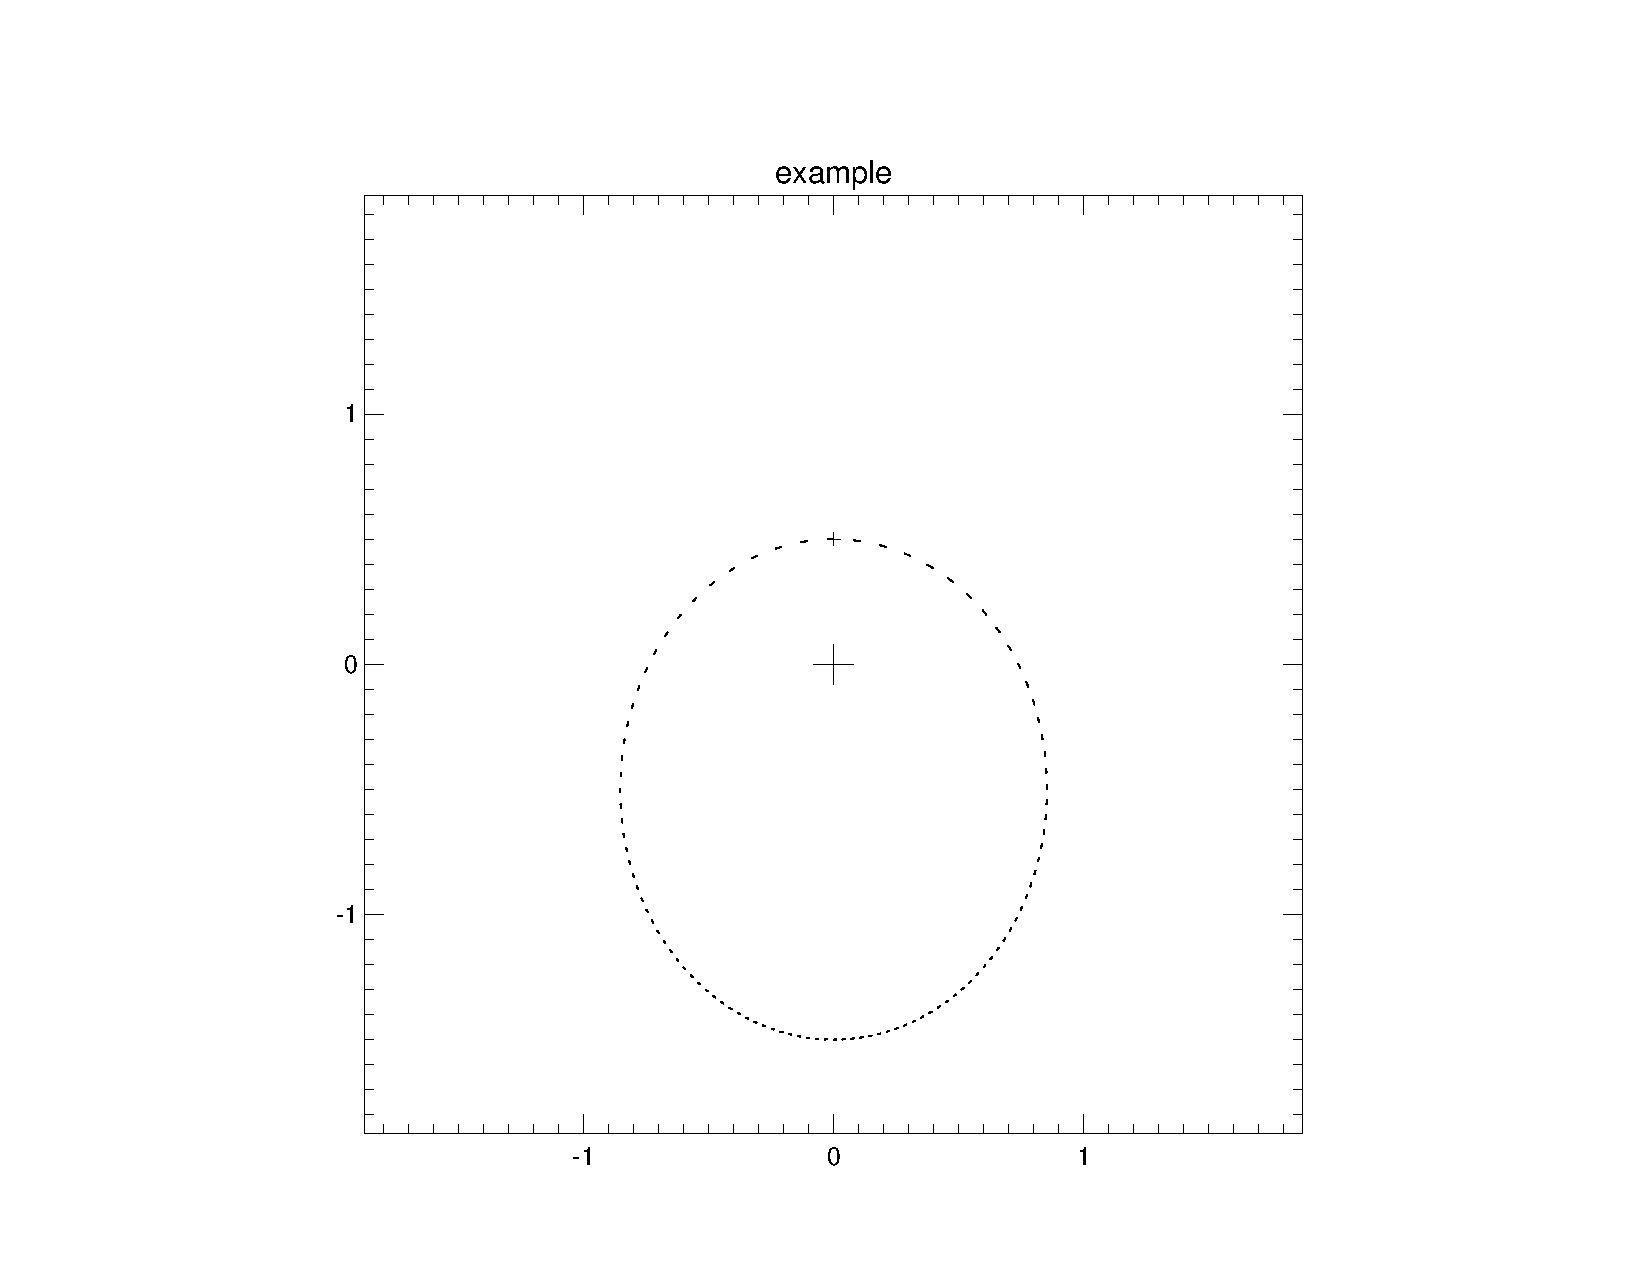
\includegraphics[angle=0,width=0.35\paperwidth]{rk_inte1_example.pdf}

\newpage

\black How does the error in energy depends on eccentricity,
timestep, and the order of integration?



\vspace{1cm}
{\bf \framebox{rk\_inte1\_eks\_taylor2.pro}}
Comparison for eks=0.1,0.3,0.5, using II degree Taylor



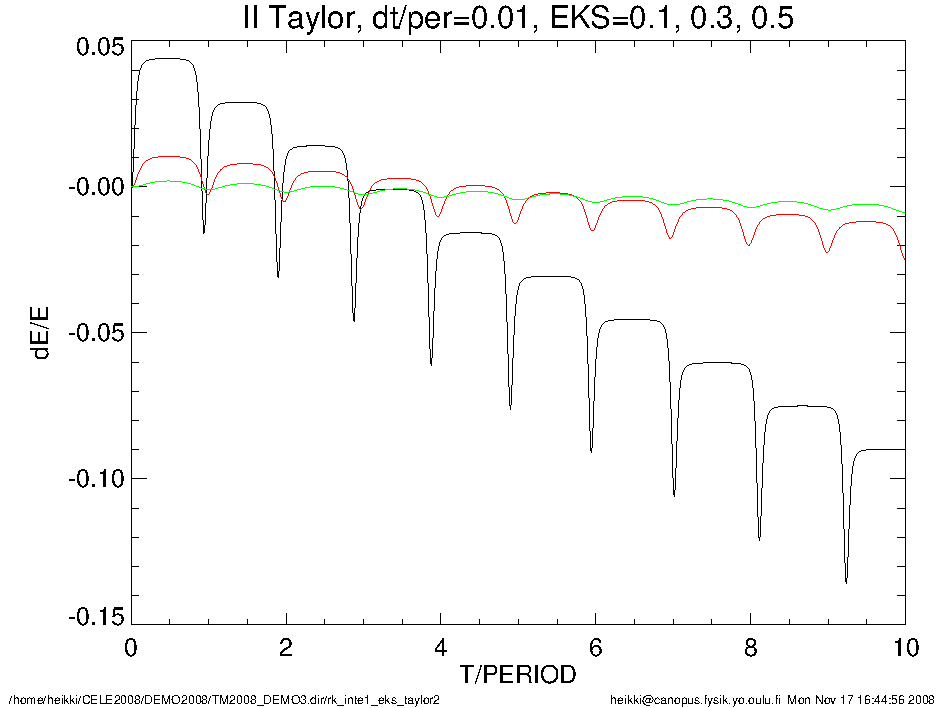
\includegraphics[width=0.5\paperwidth]{rk_inte1_eks_taylor2.pdf}



\vspace {1cm}

{\bf \framebox{rk\_inte1\_dttest\_rk4.pro}}
Check the energy error vs. time, with RK4 and two different time steps dt=0.01 and 0.001 periods (eks=0.5)

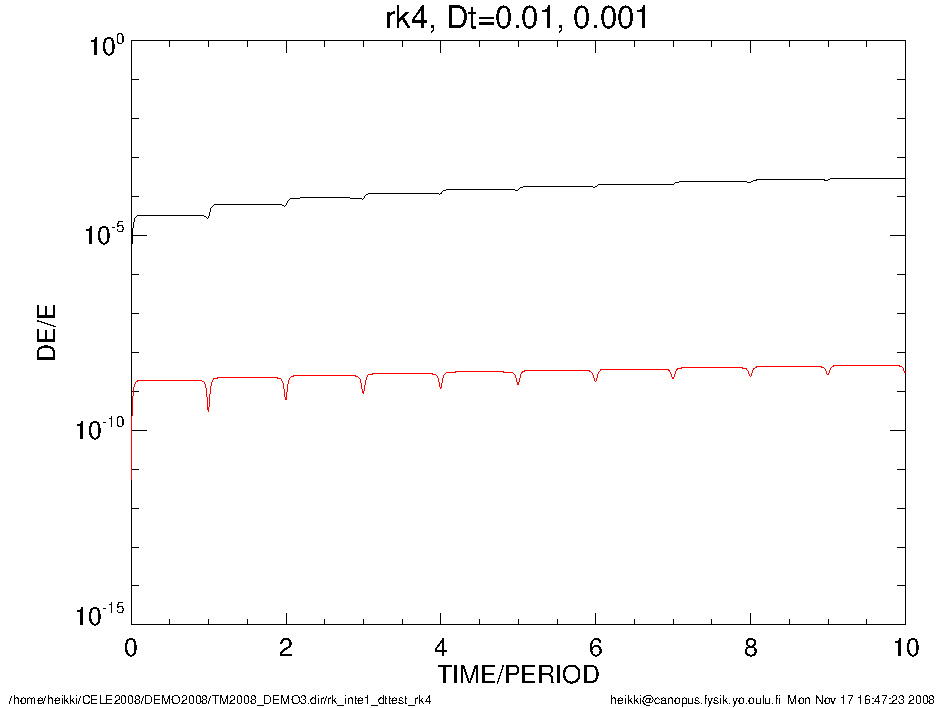
\includegraphics[angle=0,width=0.35\paperwidth]{rk_inte1_dttest_rk4.pdf}



\vspace {1cm}

\newpage

{\bf \framebox{rk\_inte1\_dttest.pro}}


The secular and maximum periodic errors are shown separately
for the case $\epsilon=0.5$. DT gives the timestep relative to orbital period


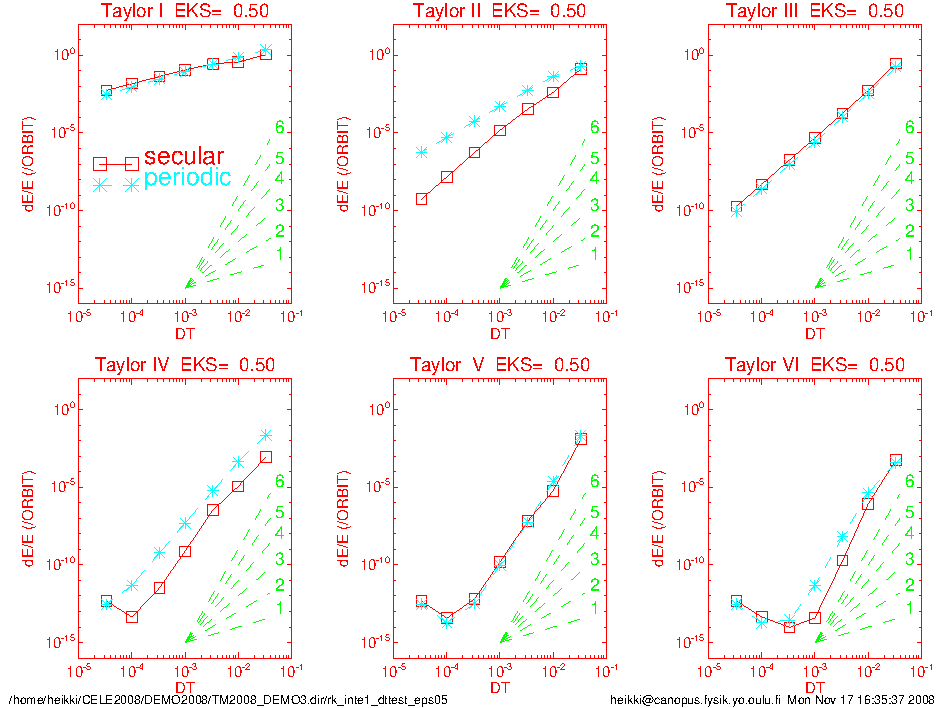
\includegraphics[width=0.75\paperwidth]{rk_inte1_dttest_eps05.pdf}








\newpage

\black
{\medb 8.3 PERTURBED TWO BODY MOTION} ({\bf inte\_perp.pro})


\hlin
\bul Add perturbation to the relative 2-body force. Perturbation has
the form used in the lectures:


\buu \buu \framebox{$\vec F = f_r {\vec R}/r  + f_v {\vec V}/v + f_n \vec N$}

\buu \buu \buu $f_r = \alpha ~ \mu/a^2$   

\buu \buu \buu $f_v = \beta ~ \mu/a^2$

\buu \buu \buu $f_n = \gamma ~ \mu/a^2$

\bul The following subroutine uses rk4 to integrate the perturbed motion.
Initial values are defined via unperturbed orbital
elements. Perturbation defined via keywords {\tt alpha, beta,
gamma}. As a default they affect continuosly: by the keywords {\tt E1,
E2} one can specify an interval during which the perturbations affect
the orbit.





{\scriptsize \red
\verbatiminput{inte_perp.pro}
}\black

{\scriptsize \red
\verbatiminput{inte_perp_func.pro}
}\black

\newpage

\black

Example: {\bf inte\_perp\_demo\_rad.pro}

\bul The effect of instantaneous radial perturbation, affecting
 at different parts of the orbit (the same plot was attached to
the lectures):

{\scriptsize \red
\verbatiminput{inte_perp_demo_rad.pro}
}\black

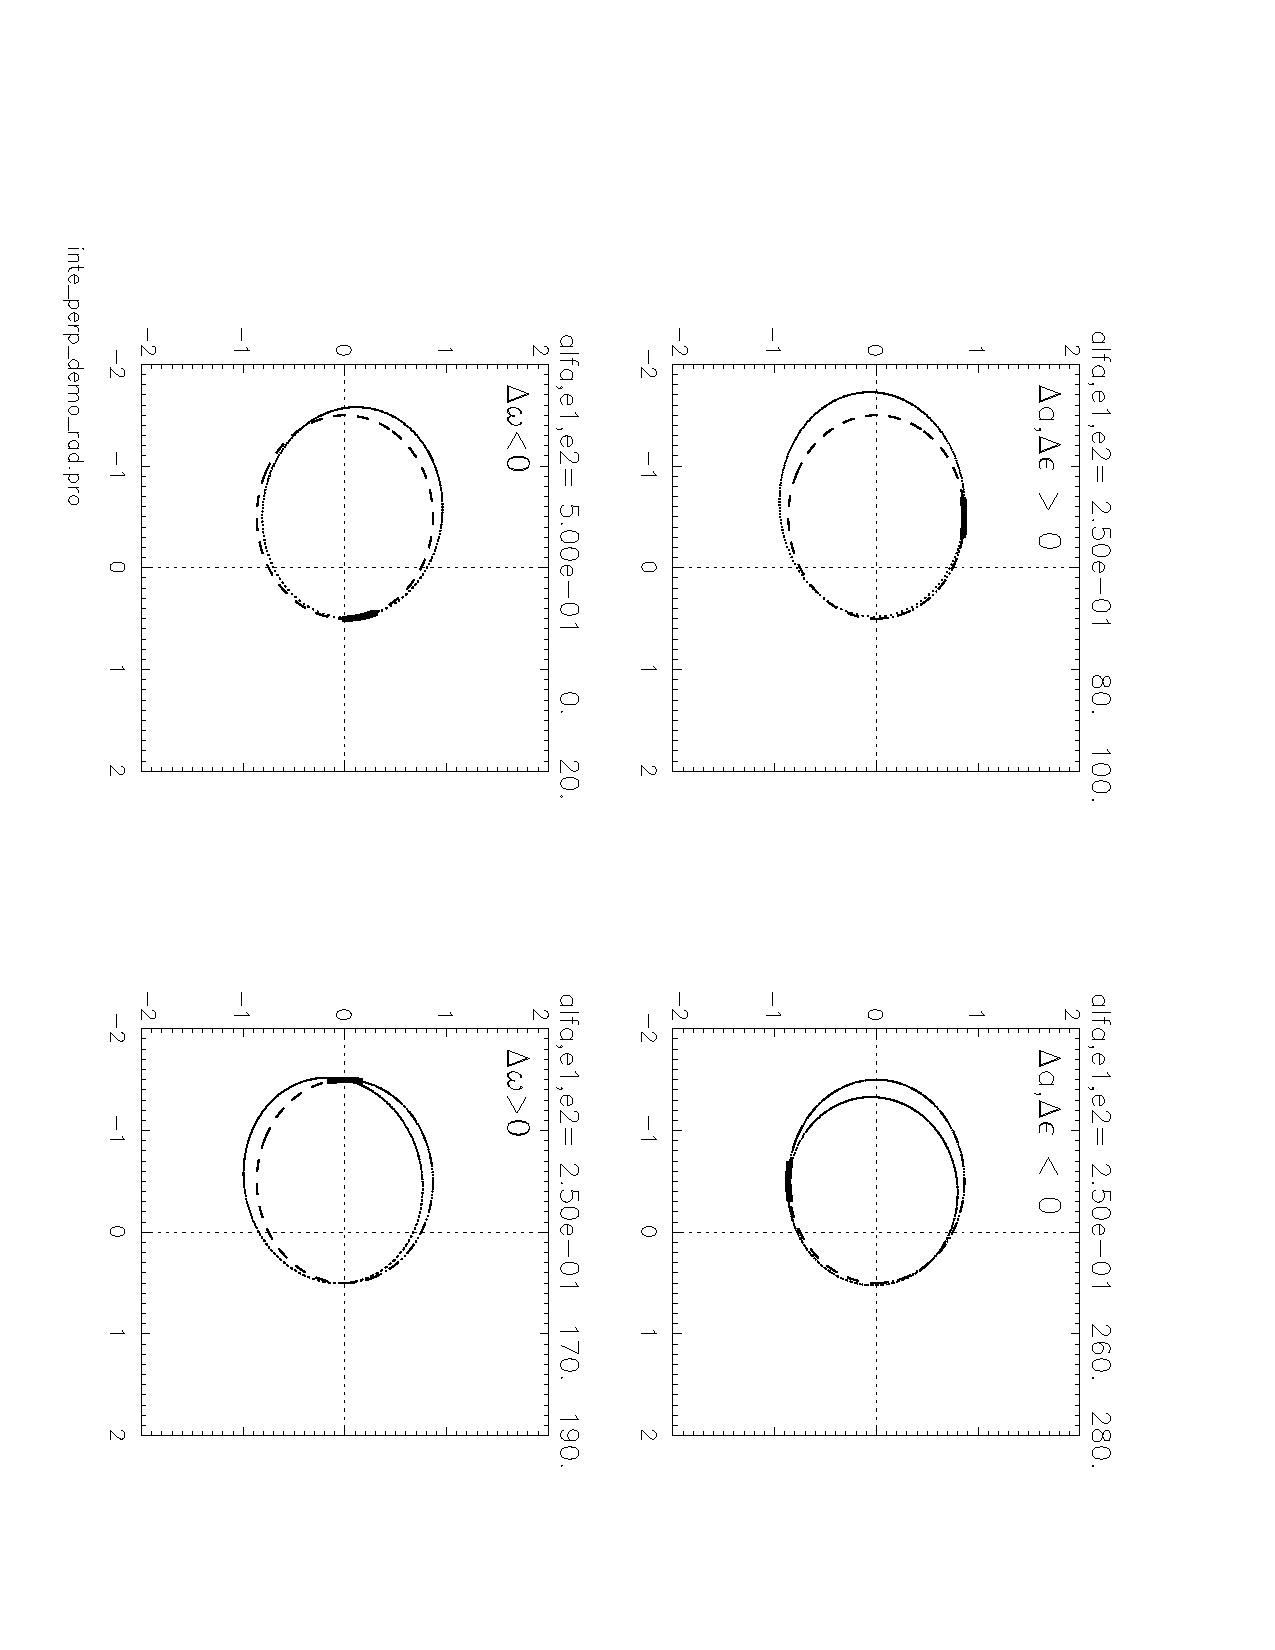
\includegraphics[angle=90,width=0.75\paperwidth]{inte_perp_demo_rad.pdf}

\newpage
\black

Example: {\bf inte\_perp\_demo\_vel.pro}

\bul The effect of instantaneous perturbation in the direction of
velocity vector, affecting at different parts of the orbit (the same
plot was attached to the lectures):

{\scriptsize \red
\verbatiminput{inte_perp_demo_vel.pro}
}\black

 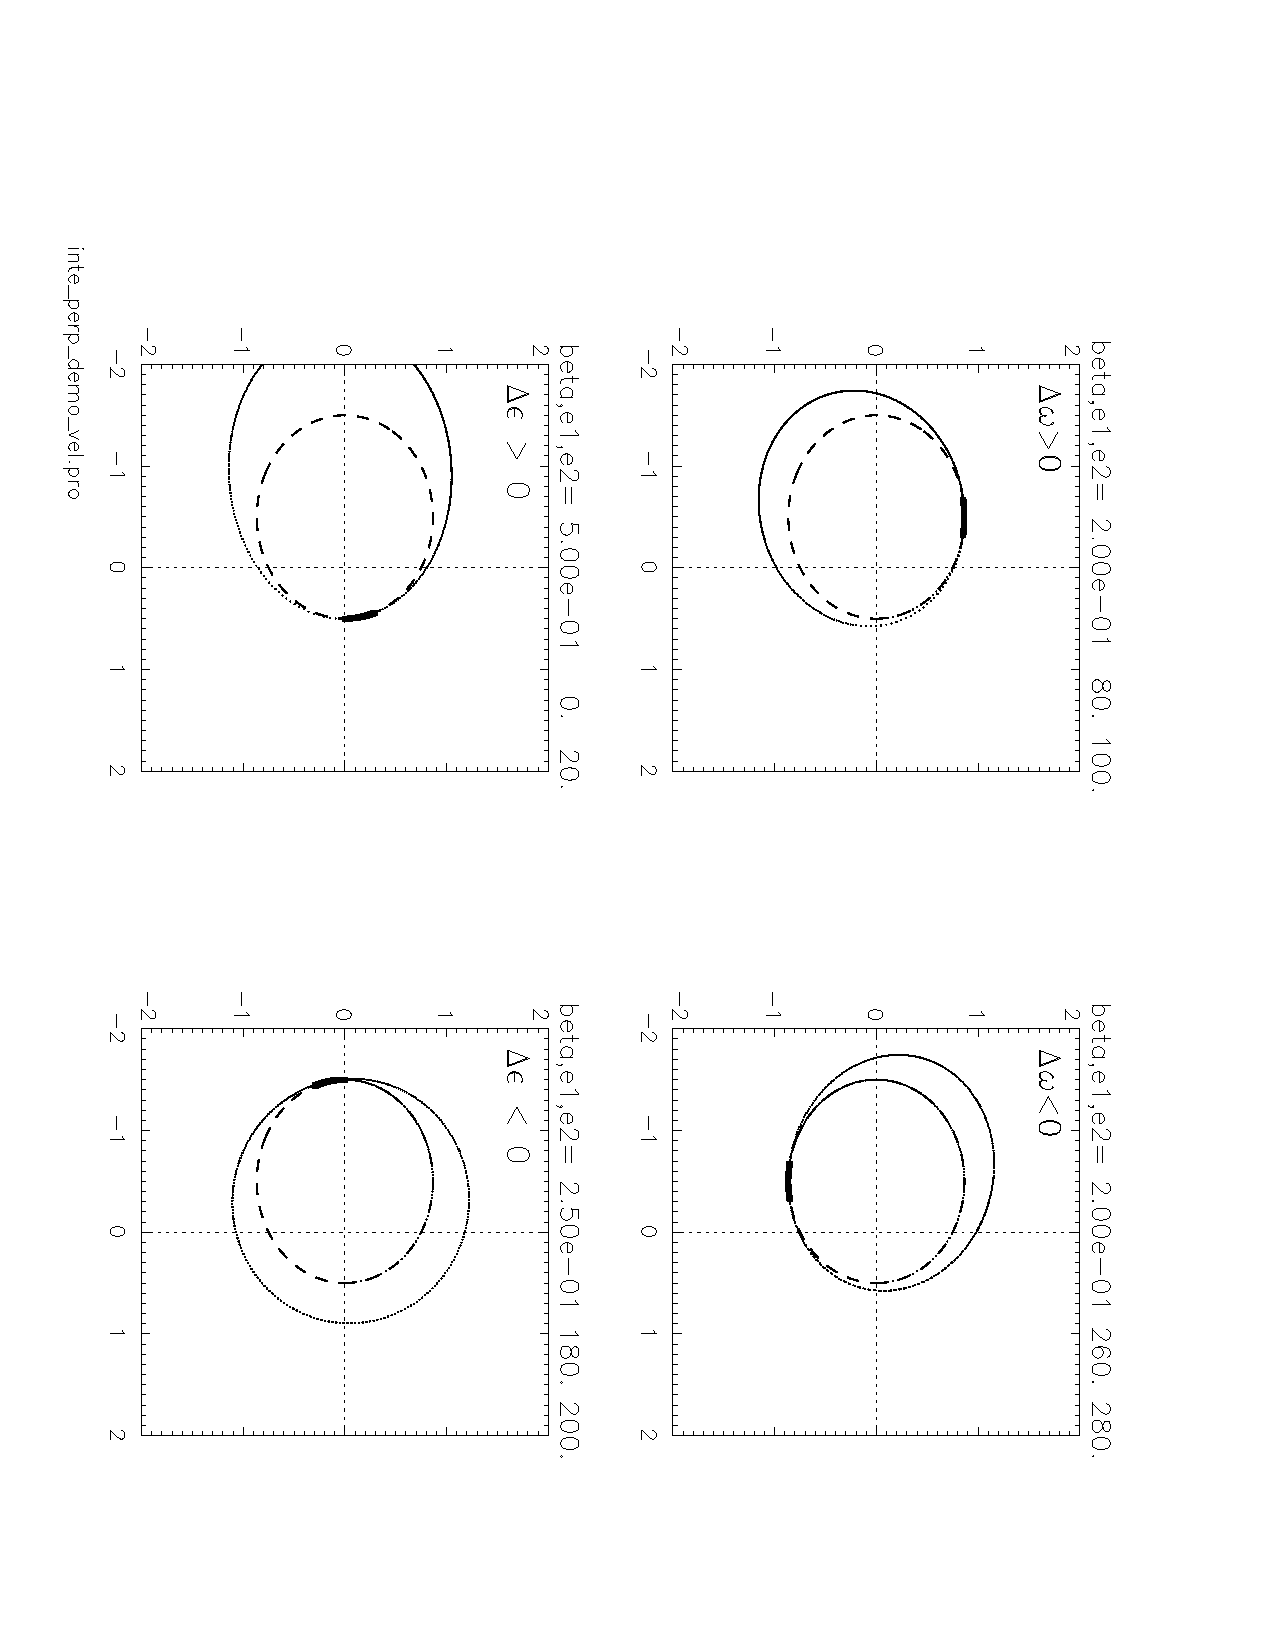
\includegraphics[angle=90,width=0.75\paperwidth]{inte_perp_demo_vel.pdf}

\newpage
\black

Example: {\bf inte\_perp\_demo\_rad2.pro}

\bul The effect of continouos radial perturbation. Comparison to
analytical formulas derived in the lectures (the same plot was
attached to the lectures):

{\scriptsize \red
\verbatiminput{inte_perp_demo_rad2.pro}
}\black

\hspace{-3cm} 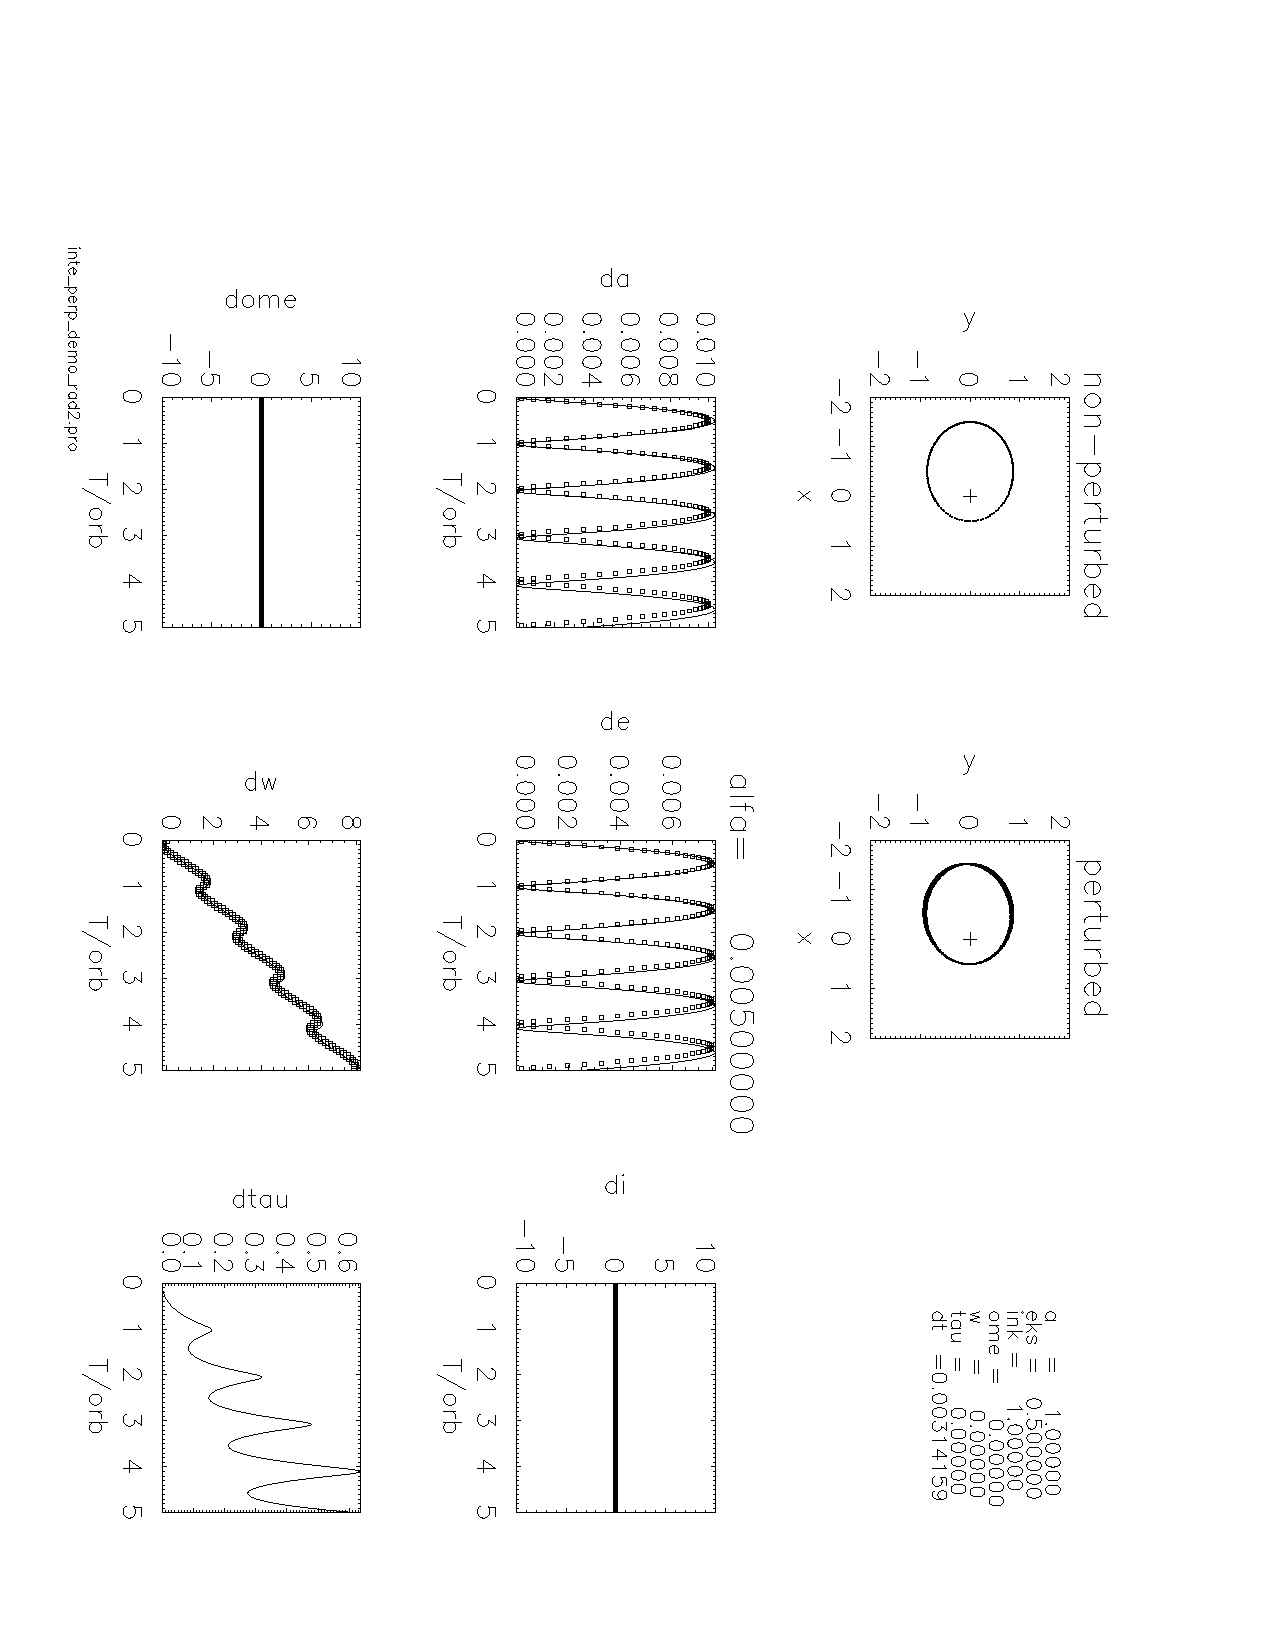
\includegraphics[angle=90,width=0.9\paperwidth]{inte_perp_demo_rad2.pdf}



\newpage
\black

Example: {\bf inte\_perp\_demo\_vel2.pro}

\bul The effect of continouos perturbation in the direction of velocity vector. Comparison to
analytical formulas derived in the lectures (the same plot was
attached to the lectures):

{\scriptsize \red
\verbatiminput{inte_perp_demo_vel2.pro}
}\black

\hspace{-3cm} 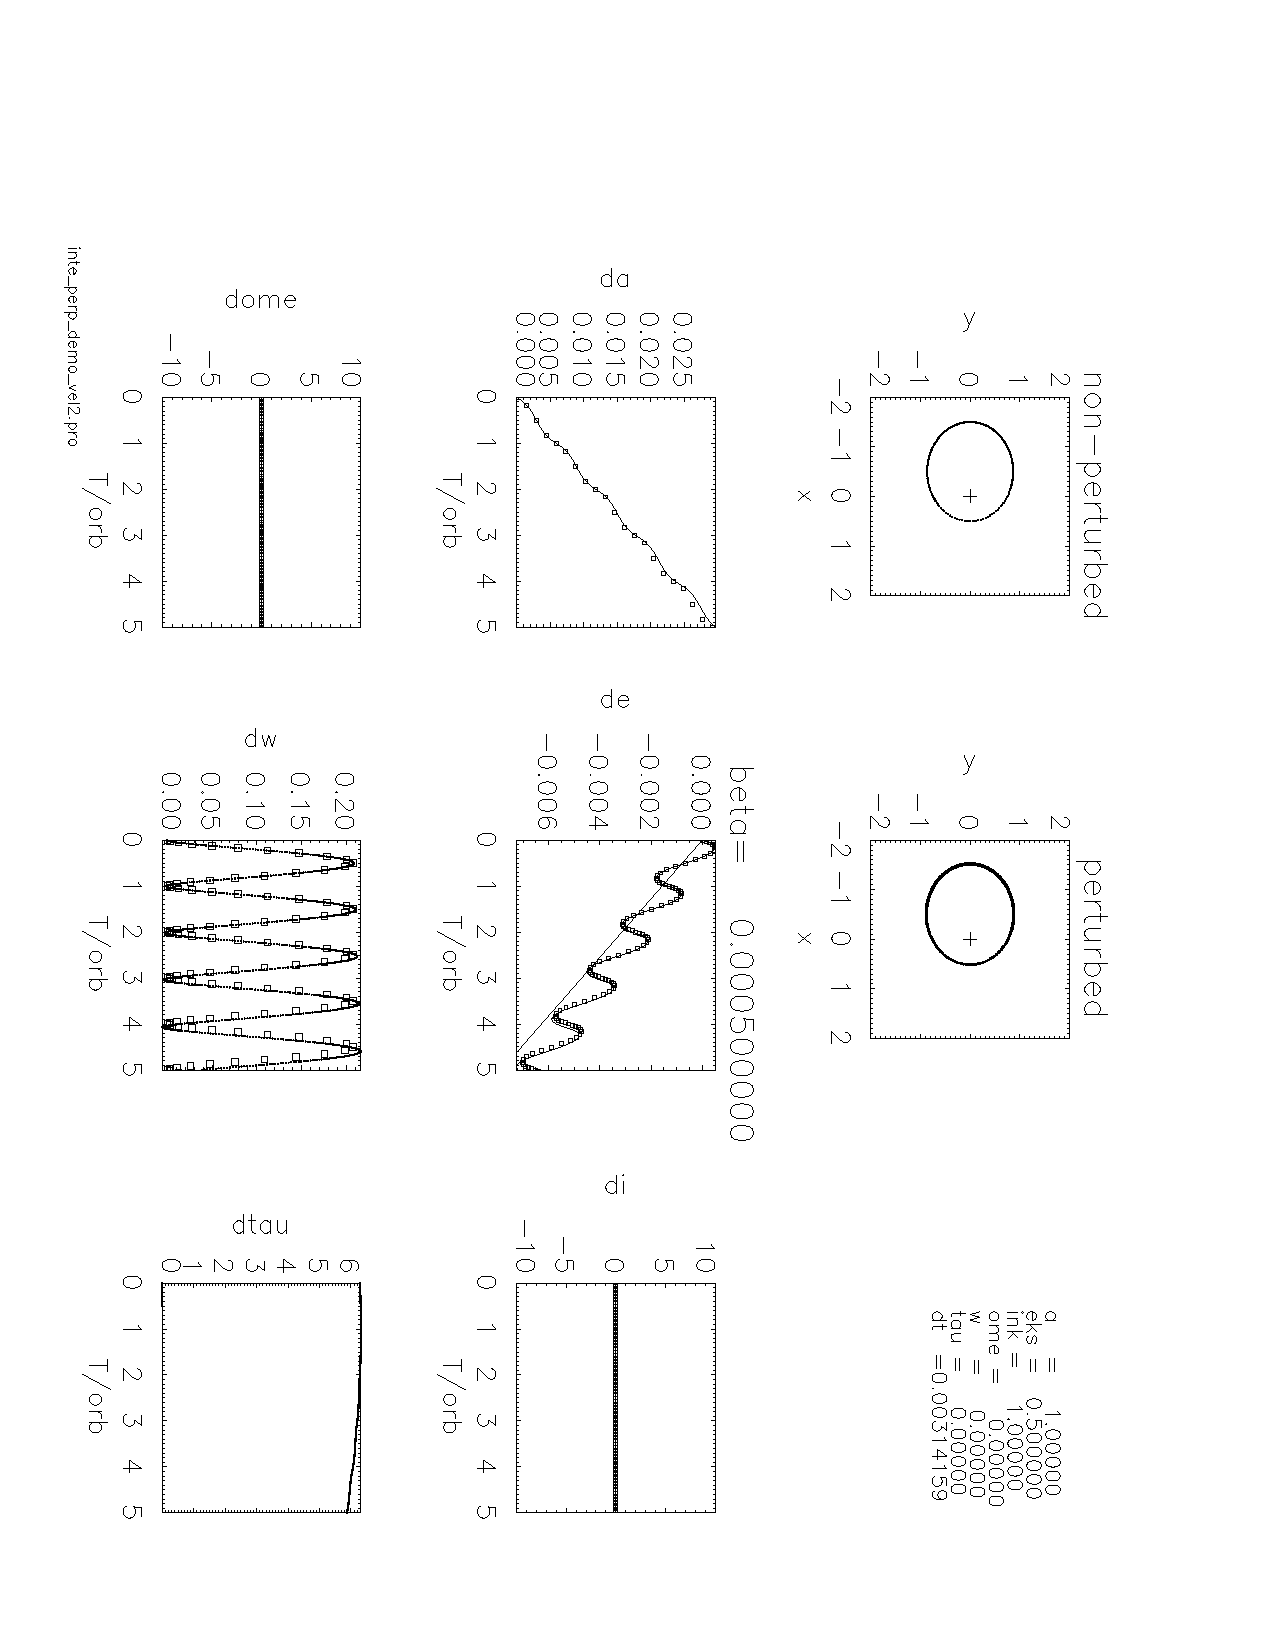
\includegraphics[angle=90,width=0.8\paperwidth]{inte_perp_demo_vel2.pdf}


\newpage
\black

Example: {\bf inte\_perp\_demo\_nor2.pro}

\bul The effect of continouos perturbation in the direction normal to
the orbit. Comparison to analytical formulas derived in the lectures
(the same plot was attached to the lectures):

{\scriptsize \red
\verbatiminput{inte_perp_demo_nor2.pro}
}\black

\hspace{-3cm} 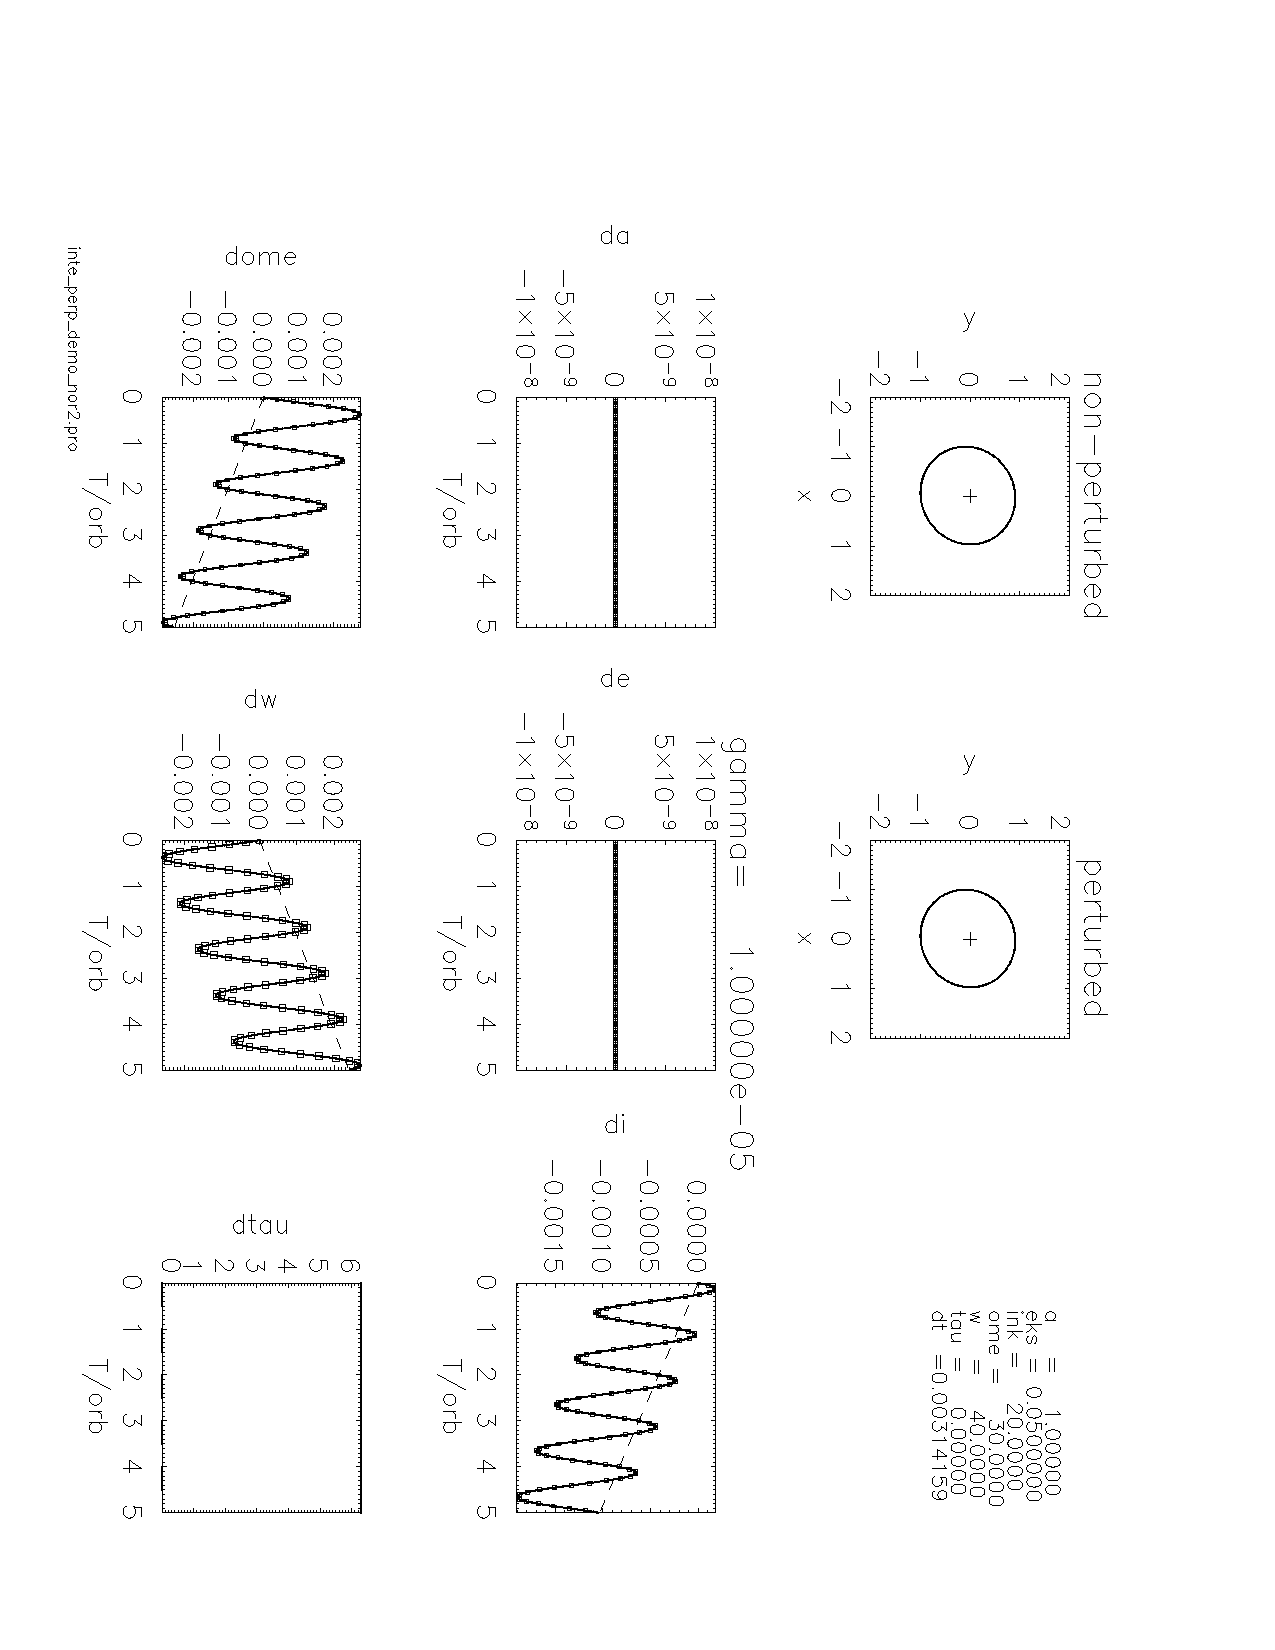
\includegraphics[angle=90,width=0.9\paperwidth]{inte_perp_demo_nor2.pdf}






\end{document}
